\chapter{設計と実装}
\label{chap:design_and_impl}
本章では,前提となる Linux カーネルにおけるパケットフォワーディング処理,netfilter に関する知識を解説し,本論文の提案手法についての設計と実装について述べる.
\section{Linux カーネルにおけるパケットフォワーディング}
\textbf{[Linux カーネルにおけるパケットフォワーディングの流れや,その実装について説明する.]}

\section{設計}
SR-Aware NF の新しい実装として,Linux のルーティングインフラに netfilter によるパケットのフィルタリングとマングリング機能を統合した SRv6 End ビヘイビアである End.AN.NF を提案する.
End.AN.NF は,End behavior of SR-Aware Native function for NetFilter の略である.
End.AN.NF の実装は,Linux カーネルの IPv6 ルーティングスタックを活用するように設計されている.
End.AN.NF の SID は IPv6 アドレスとして表現され,Linux 上では IPv6 ルーティングテーブルエントリとして扱われる.
End.AN.NF を示す SID は,通常の IPv6 経路として既存のルーティングプロトコル,及びその実装を介して他のノードに透過的に広告される.
さらに,End.AN.NF では,SRv6 でカプセル化されたインナーパケットに対して,netfilter のルールを適用できる.
End.AN.NF は,nftables\cite{nftables} や iptables~\cite{iptables} を介して設定されたトラフィックに対する選択的なパケット破棄や NAT の適用などを SRH でカプセル化された内部のパケットに対して適用できる.
また,nftables や iptables に限らず,その他の netfilter ベースのアプリケーションについても,それらの実装を変更することなく SR-Aware NF として使用可能にする.

Netfilterは,Linuxのレイヤ3パケット転送フローに3つのフックポイントを持ち,異なるタイミングでパケットに netfilter ルールを適用する.
図\ref*{fig:hooks} は,トランジットパケットに適用される netfilter のフックのフローを示している.
受信したあるパケットに対して End.AN.NF が動作する際,そのパケットは 2 段階の netfilter フックが適用される.
1つ目の適用では,SRH を含む外部 IPv6 ヘッダのついたカプセル化されたパケットに対して,その外部 IPv6 ヘッダをターゲットにして実行される.
2つ目の適用では,SRH を含まない,カプセル化された内部パケットの IP ヘッダをターゲットにして実行される.
まず,End.AN.NF を実装した Linux ベースの SRv6 ノードが IPv6 パケットを受信すると,そのカーネルは受信したパケットに prerouting フックを適用し,通常通り宛先 IPv6 アドレスの最長プレフィックスマッチングを行う.
宛先アドレスがローカルの End.AN.NF の SID である場合,カーネルはパケットを End.AN.NF の実装に渡し,そうでない場合,カーネルは forward フックと postrouting フックを適用しながら,IPv6 パケットを対応するネクストホップに転送する.
一方,End.AN.NF は,SRHでカプセル化されたインナーパケットに対して,再度,prerouting フック,forward フック,及び postrouting フックを適用する.
End.AN.NF の段階で netfilter が適用されている間,SRH は End.AN.NF によって隠されるので,netfilter は SRH の処理を考慮する必要がない.
End.AN.NF が終了すると,外部 IPv6 ヘッダの宛先アドレスは次の SID に置き換えられ,カプセル化されたパケットは Linux の IPv6 パケットフォワーディングプロセスにおける通常の転送パスに戻る.

End.AN.NF は,パケットをマーキングするために SID の \texttt{ARG} フィールドを利用する.
ARG は SID の下位ビットである~\cite{rfc8986}.
SRv6 の仕様では,ある End ビヘイビアがその End ビヘイビア固有の用途で \texttt{ARG} を利用することを許可している.
End.AN.NF では,SID の ARG がマークとして Linux カーネル空間におけるパケットバッファに付加される.
netfilter ベースのアプリケーションは,パケットバッファ上のマークを照合することで,適用するルールを変更することができる.
したがって,オペレータが,単一の End.AN.NF SID しか定義されていない場合であっても,NF は ARG に基づいてトラフィックのルールを調整することが可能である.

アルゴリズム~\ref*{alg:end-an-nf} は,End.AN.NF がパケットを netfilter のフックポイントに渡す方法を示した擬似コードである.
まず,End.AN.NF は,ARG の長さがこの End.AN.NF SID に指定されている場合,受信したパケットの宛先アドレスから ARG 値を抽出する.
抽出された ARG 値は,マークとしてパケットバッファに付加される.
次に,End.AN.NF はパケットバッファの先頭を外側の SRH から内側のパケットに切り替え,バッファを netfilter フックに渡す.
フックにインストールされたルールが内側のパケットに適用された後,End.AN.NF は,パケットバッファの先頭を内側のパケットから外側の SRH に復元し,パケットを次のプロセスに渡す.
この手順は,図~\ref*{fig:hooks} の赤い長方形で示した3つのフックポイント,prerouting,forward,postrouting に対してそれぞれ適用する.

Linux カーネルは,End ビヘイビアを関数の SID を宛先とするルーティングテーブルエントリとして実装している.
このメカニズムは seg6local と呼ばれる.
End.AN.NF は End ビヘイビアの1つであるため,その実装も seg6local を利用している.
図~\ref*{fig:show-route} に示すように,カーネルは他の End ビヘイビアと同様に End.AN.NF を表す SID をルーティングテーブルエントリとして扱っていることが確認できる.
ルーティングソフトウェアや iproute2 を用いて SID をルーティングテーブルエントリとして追加すると,従来のルーティングプロトコルを用いてカーネルのルーティングテーブルにインストールされた経路を広告することが可能となる.
実際に FRRouting~\cite{frr} を使用し,カーネル内の End.AN.NF に関連付けられた SID を BGP 経由で他のルータに IPv6 経路として広告できることを確認した.
End.AN.NF のアーキテクチャは,ルーティング制御に既存のルーティングプロトコルを使用できるため,既存の NF との互換性が高い.
このアーキテクチャは,Linux netfilter を用いた SR-Aware NF の実現方法の一つである.

\begin{figure}[t]
    \centering
    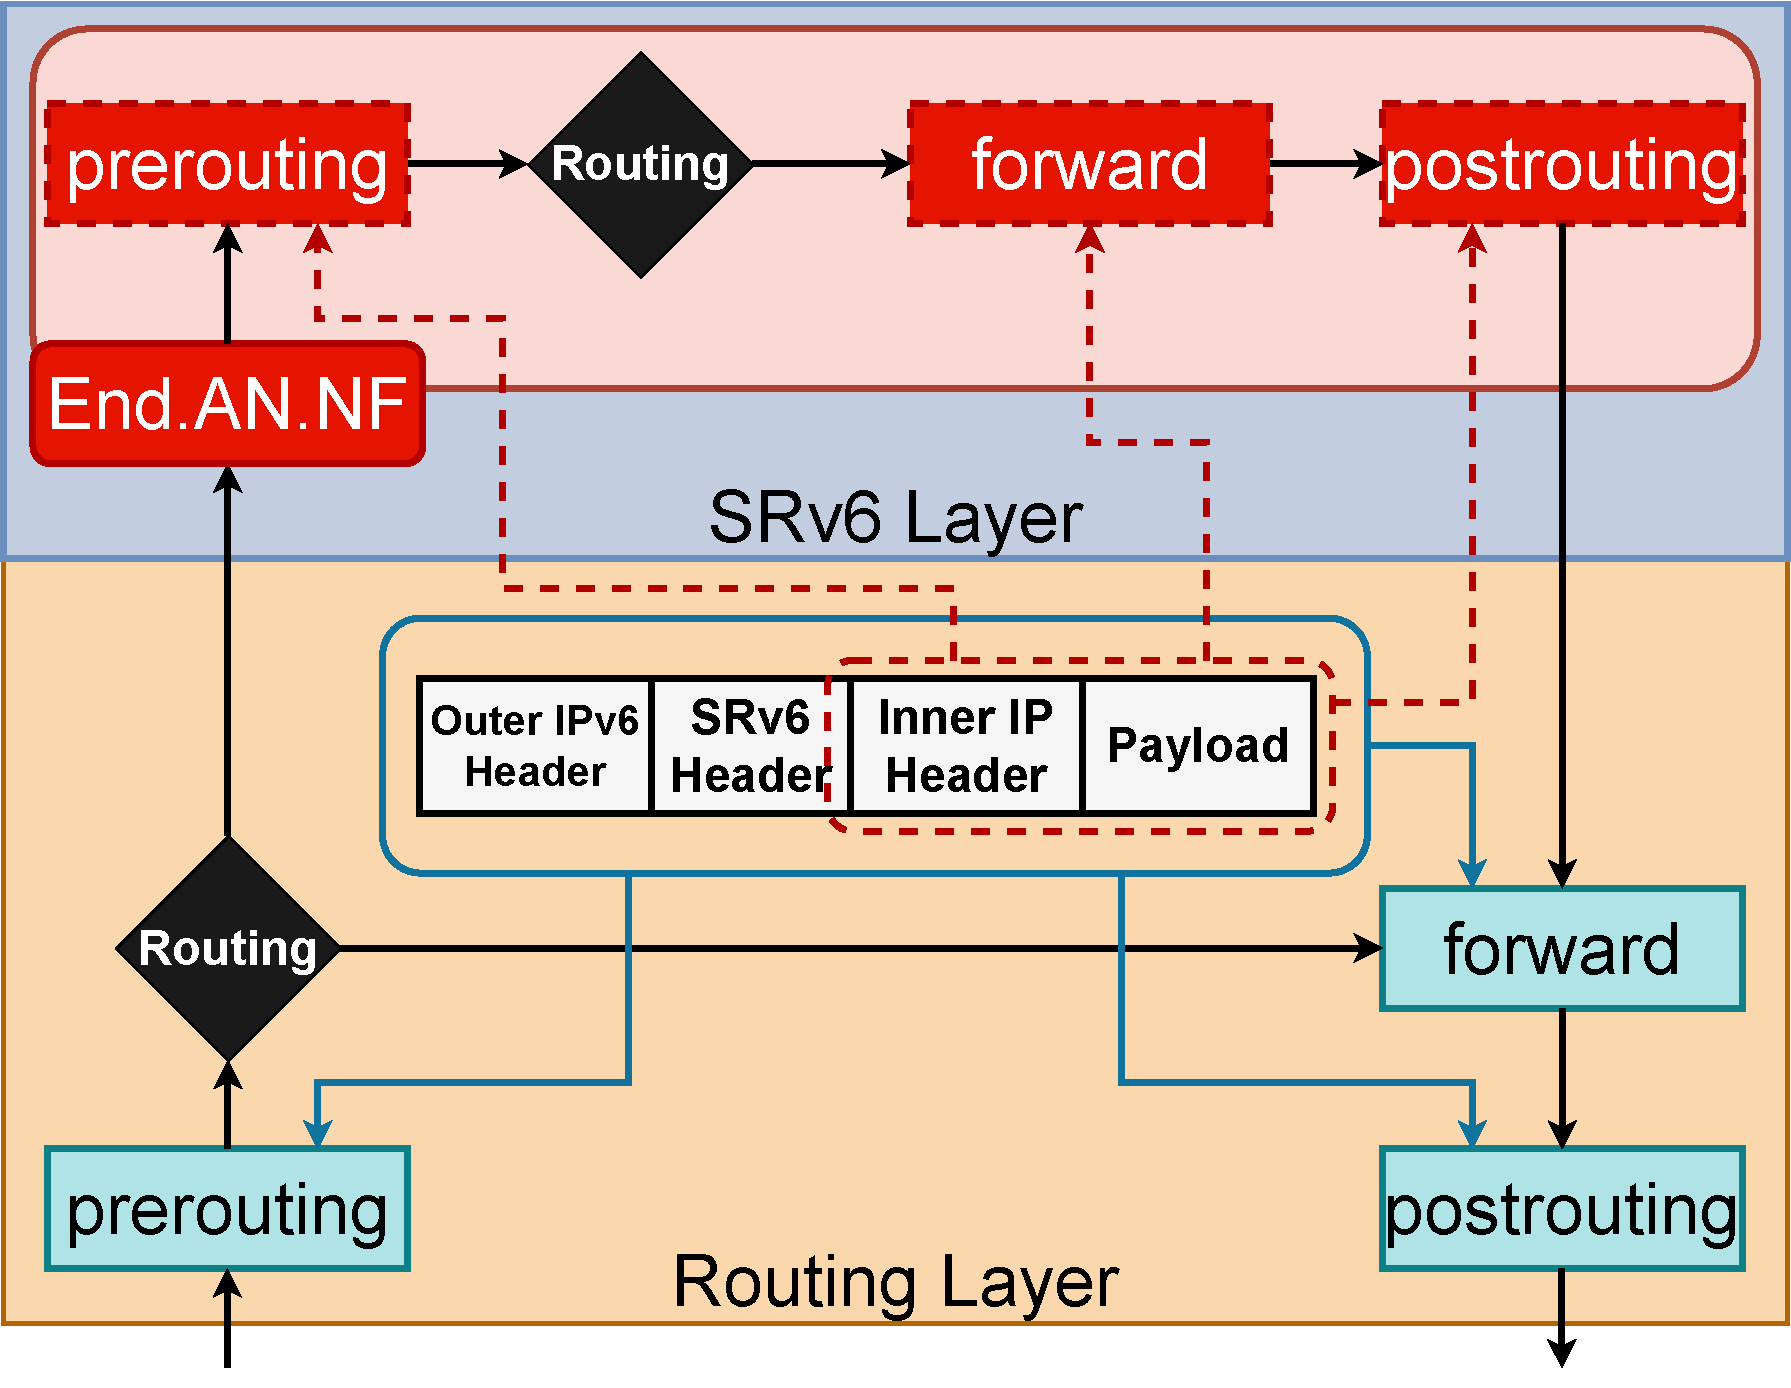
\includegraphics[
      width=0.95\linewidth,
      keepaspectratio=true
    ]{img/End-AN-NF-hooks.pdf}
    \caption{\texttt{End.AN.NF} applies three netfilter hook points, prerouting, forward, and postrouting, to inner packets encapsulated in SRv6.}
    \label{fig:hooks}
  \end{figure}
  
  \begin{algorithm*}[t]
    \caption{Pseudo code of passing a packet to a netfilter hook point in \texttt{End.AN.NF}}
    \small
    \label{alg:end-an-nf}
    \begin{algorithmic}[1]
      \if 0
      \Function {Process\_End.AN.NF}{$packet$}
      \State Call function \textbf{Pass\_to\_Hook} with following args: ($packet$, prerouting)
      \State Decrement segleft by 1
      \State Rewrite destination address based on the SID list and segleft, in the SID of the $packet$
      \State Lookup next hop in th routing table entry for rewrite new destination address
      \State Call function \textbf{Pass\_to\_Hook} with following args: ($packet$, forward)
      \State Call function \textbf{Pass\_to\_Hook} with following args: ($packet$, postrouting)
      \EndFunction
      \fi
      % \Function {Pass\_to\_Hook}{$packet$, $hook\_point$}
      \Function {PassPacketToHook}{$packet$}
      \If {the length of $ARG$ is specified for this \texttt{End.AN.NF} SID}
      \State Extract the $ARG$ value from the destination address of outer SRH
      \State Mark the $ARG$ value on the packet buffer $packet$
      \EndIf
      \State Switch the head of packet buffer $packet$ from the outer SRH to the inner packet
      \State Pass $packet$ to a netfilter hook
      \State Switch the head of packet buffer $packet$ from the inner packet to the outer SRH
      \EndFunction
    \end{algorithmic}
  \end{algorithm*}
  
  \begin{figure*}[t]
    \centering
    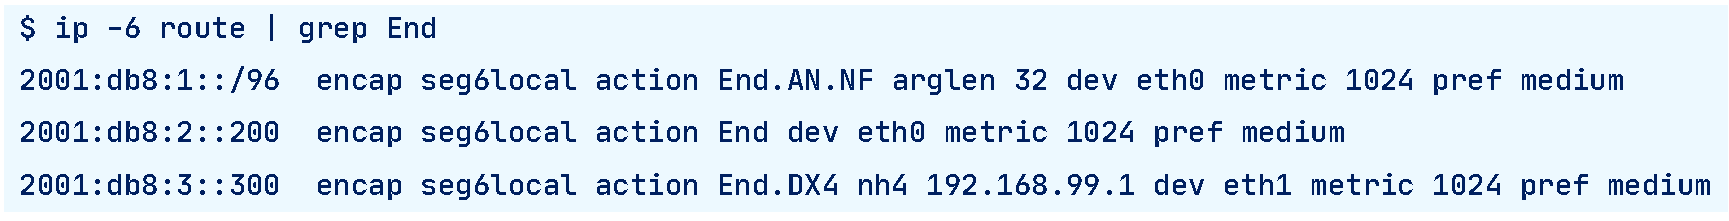
\includegraphics[width=0.95\linewidth]{img/End-FW-show-route.pdf}
    \caption{The modified Linux kernel treats an \texttt{End.AN.NF} SID as an IPv6 routing table entry. We can manage the \texttt{End.AN.NF} routes with the existing tools such as iproute2.}
    \label{fig:show-route}
  \end{figure*}